\documentclass[twocolumn]{aastex62}
\usepackage{graphicx}
\usepackage{subfigure}

\newcommand{\vdag}{(v)^\dagger}
\newcommand\aastex{AAS\TeX}
\newcommand\latex{La\TeX}

%% Reintroduced the \received and \accepted commands from AASTeX v5.2
%% Command to document which AAS Journal the manuscript was submitted to.
%% Adds "Submitted to " the arguement.
\submitjournal{ApJ}

\def\ie{{\it i.e. }}
\def\eg{{\it e.g. }}

\shorttitle{Include the Extreme Faint Galaxy in Shear Measurement}
\shortauthors{Hekun Li et al.}


\begin{document}

\title{Include the Extreme Faint Galaxy in Shear Measurement}


\correspondingauthor{Jun Zhang}
\email{betajzhang@sjtu.edu.cn}

\author{Hekun Li}
\affiliation{Department of Physics and Astronomy, Shanghai Jiao Tong University, Shanghai 200240, China}
\author{Jun Zhang*}
\affiliation{Department of Physics and Astronomy, Shanghai Jiao Tong University, Shanghai 200240, China}


\begin{abstract}



\end{abstract}


\keywords{gravitational lensing: weak-methods: data analysis}


\section{Introduction} \label{sec:intro}
noise bias, SNR threshold

precision achieved

cite the previous paper, cut and calibration to avoid bias

introduce some aspects of Fourier\_Quad and PDF\_SYM

recently, we found small bias on the faint end

multiplicative \& additive bias of these methods
\section{Approach the sub-percent level accuracy}
\subsection{The Fourier\_Quad method}\label{sec:FQ}
%introduce the details of shear measurement, average approach
The Fourier\_Quad is a model-independent shear measurement method which estimates the shape of galaxy based on its 2D power spectrum \citep{Zhang2008, Zhang2015, Zhang2017}. The shear estimators are defined as:
\begin{eqnarray}
\label{shear_estimator}
G_1&=&-\int d^2\vec{k}(k_x^2-k_y^2)T(\vec{k})M(\vec{k})\\ \nonumber
G_2&=&-2\int d^2\vec{k}k_xk_yT(\vec{k})M(\vec{k})\\ \nonumber
N&=&2\int d^2\vec{k}\left[k^2-\frac{\beta^2}{2}k^4\right]T(\vec{k})M(\vec{k}), \\ \nonumber
U &=& -\beta^2\int d^2\vec{k}(k_x^4 - 6k_x^2k_y^2 + k_y^4)T(\vec{k})M(\vec{k}), \\ \nonumber
V &=& -4\beta^2\int d^2\vec{k}(k_x^3k_y - k_xk_y^3)T(\vec{k})M(\vec{k}).
\end{eqnarray}
The $M(\vec{k})$ is the power spectrum of the galaxy image from which the background and Poisson noise have been subtracted through:
\begin{eqnarray}
\label{FQ_TM}
&&M(\vec{k})=\left\vert\widetilde{f}_S(\vec{k})\right\vert^2-P_S-\left\vert\widetilde{f}_B(\vec{k})\right\vert^2+P_B\\ \nonumber
&&P_S=\frac{\int_{\vert\vec{k}\vert > k_c} d^2\vec{k}\left\vert\widetilde{f}_S(\vec{k})\right\vert^2}{\int_{\vert\vec{k}\vert > k_c} d^2\vec{k}}, \;\;\; P_B=\frac{\int_{\vert\vec{k}\vert > k_c} d^2\vec{k}\left\vert\widetilde{f}_B(\vec{k})\right\vert^2}{\int_{\vert\vec{k}\vert > k_c} d^2\vec{k}},
\end{eqnarray}
where $\widetilde{f}_S(\vec{k})$ and $\widetilde{f}_B(\vec{k})$ are the Fourier transformations of the galaxy image and a neighboring image of background noise respectively. $P_B$ and $P_S$ are the estimates of the Poisson noise power spectrum of the background noise and source images respectively. A critical wavelength, $k_c$, is required to avoid the contamination of the source power\citep{Zhang2015}. The factor $T(\vec{k})$ is the ratio of power spectrum of the target isotropic Gaussian PSF (point spread function) to that of the original PSF, $T(\vec{k}) = |\widetilde{W}_{\beta}(\vec{k})|^2/|\widetilde{W}_{P}(\vec{k})|^2$.
It is designed to coverts the original PSF, $W_{P}(\vec{x})$, to an isotropic Gaussian PSF, $W_{\beta}(\vec{x})$, so that the effect of PSF can be corrected rigorously and model-independently.
%\begin{equation}
%W_{\beta}(\vec{x})=\frac{1}{2\pi \beta^2}\exp\left[-\frac{|\vec{x}|^2}{2\beta^2}\right]
%\end{equation}
The scale radius, $\beta$, of $W_{\beta}(\vec{x})$ should be chosen slightly larger than that of $W_{P}(\vec{x})$ to avoid the singularities in the factor $T(\vec{k})$. 

Fourier\_Quad method provides two statistical approaches for shear recovery from the estimators, the average approach and the PDF\_SYM approach. The former approach recovers the shear signal by taking ensemble averages of the shear estimators:
\begin{eqnarray}
\label{mean}
\frac{1}{2}\frac{\left\langle  G_1\right\rangle }{\left\langle  N\right\rangle }=g_1+O(g_{1,2}^3),\;\;\;\frac{\left\langle  G_2\right\rangle }{\left\langle  N\right\rangle }=g_2+O(g_{1,2}^3).
\end{eqnarray}
It is precise to the second order of shear in accuracy\citep{Zhang2015}. \cite{Zhang2015} have shown the appealing advantage of Fourier\_Quad that including the extreme faint sources or even point sources would not bias the shear measurement. However, an appropriate weight should be considered in Eq.\ref{mean} because the bright galaxies will dominate in the ensemble average and enlarge the estimate of error bar.

To approach the lower statistical error bound, \cite{Zhang2017} propose a new shear recovery method in the Fourier\_Quad framework which is called the PDF\_SYM approach. It recovers the shear signal by symmetrizing the probability distribution function (PDF) of the shear estimators. \cite{Zhang2017} show that the PDF of $\hat{G}_{1/2}$ would be maximally symmetrical respect to zero if the shear estimate, $\hat{g}_{1/2}$ is the true one (see the Ref. for more details). 
\begin{eqnarray}
\hat{G}_{1} &=& G_1 - \hat{g}_{1}(N + U) = \int d^2\vec{k} P_k T(\vec{k})M(\vec{k}), \\ \nonumber
\hat{G}_{2} &=& G_2 - \hat{g}_{2}(N - U) = \int d^2\vec{k} Q_k T(\vec{k})M(\vec{k}),\\ \nonumber
P_k &=& k_x^2-k_y^2 + \hat{g}_1\left[2k^2-\beta^2\left(k^4+k_x^4-6k_x^2k_y^2+k_y^4\right)\right],\\ \nonumber
Q_k &=& 2k_xk_y+\hat{g}_2\left[2k^2-\beta^2\left(k^4-k_x^4+6k_x^2k_y^2-k_y^4\right)\right].
\end{eqnarray}
It needs two additional shear estimators, $U$ and $V$. The $V$ term is kept for the rotation with $U$. The PDF\_SYM approach estimates each component of shear ($g_1$ or $g_2$) independently. Therefore, when estimating one component, it is convenient to ignore the other one or set it zero.   

Unlike the weighted sum of shear estimators used by the other methods, the PDF\_SYM approach includes the full PDF of the shear estimators and do not weight down the faint sources. Therefore, it could make full use of the additional information from faint sources to achieve a lower statistical error. The PDF\_SYM approach would be a promising method for shear recovery in the Fourier\_Quad framework.

Recently, we find the PDF\_SYM approach would be biased by the very faint galaxies. Figure \ref{fig:pts_mc} shows the multiplicative and additive bias from the sample of different SNR. The multiplicative bias would increase to about $1\%$ level when the SNR is about $10$. If the PSF has some anisotropy ($e \sim 0.1$), we could also find additive bias ($\sim 6\times 10^{-4}$) at the same SNR level. However, the average approach is immune to this bias even applied to the extreme noisy sample. 


% While $\sim 1\%$ bias has been found at the very faint end, it would not be a serious problem for the real measurement that includes samples from faint to bright. The result of a more realistic simulation will be shown in Section \ref{sec:improve}.


\begin{figure*}[htbp]
	\centering
	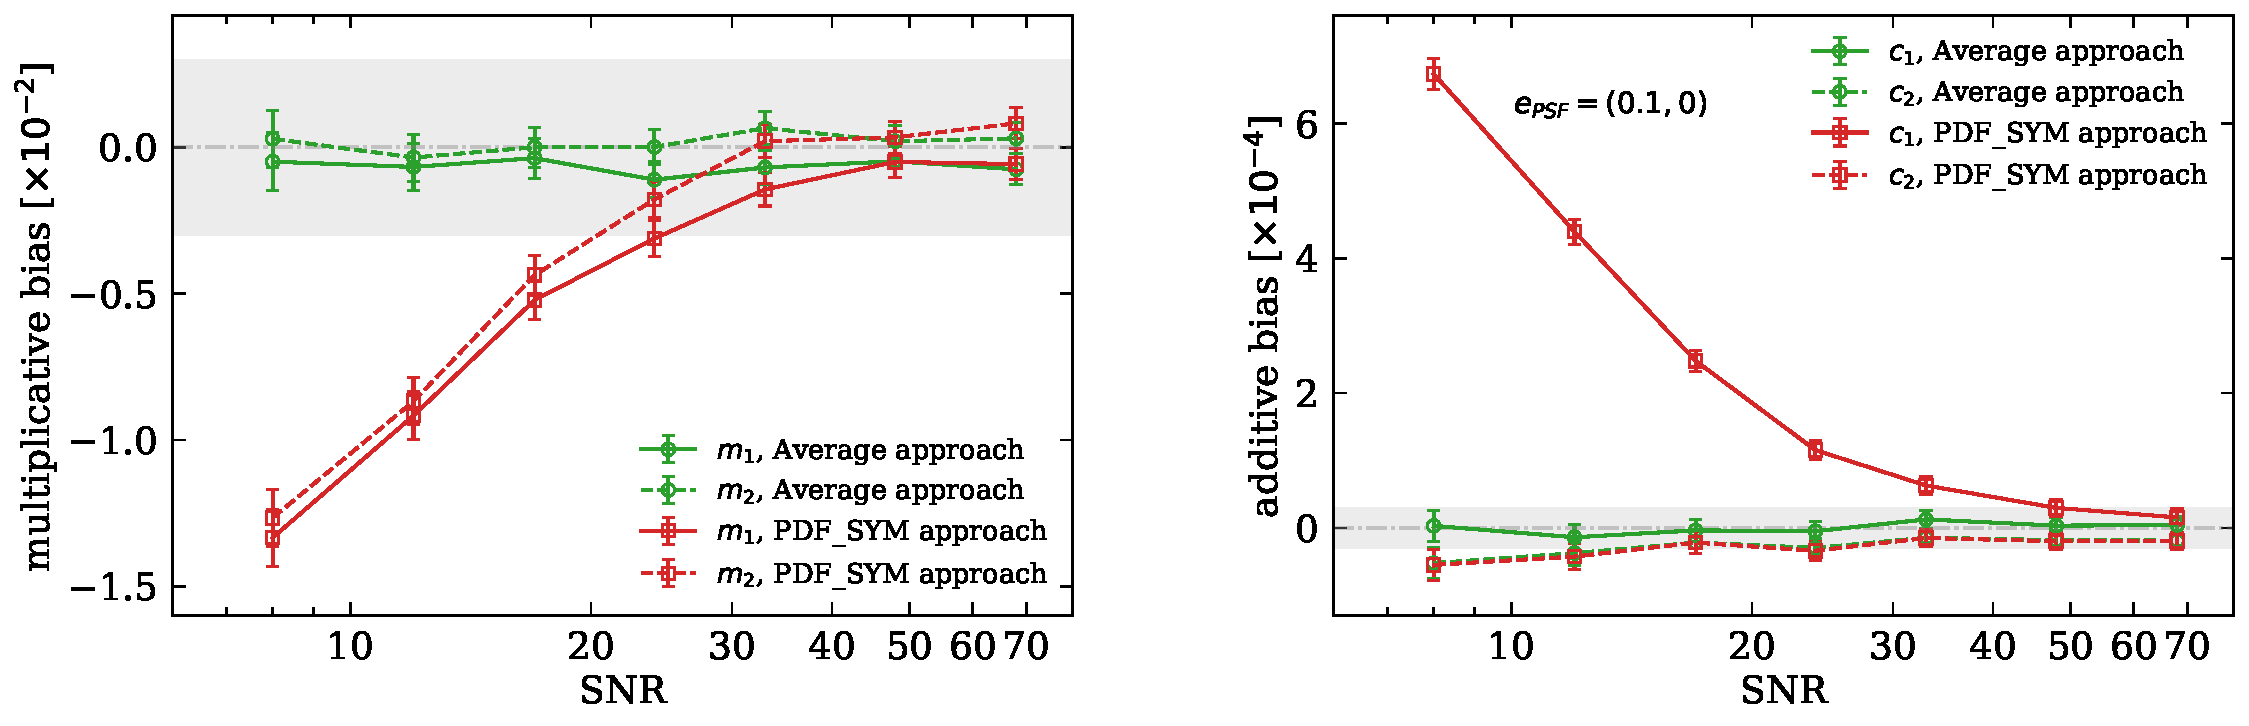
\includegraphics[width=0.9\linewidth]{figures/pts_sample_mc.pdf}
	\caption{The multiplicative and additive bias measured from the galaxy of different SNR level. The shaded region in the left (right) panel is between $\pm 3\times 10^{-3}$ ($\pm 3\times10^{-5}$) which is the fluctuation allowed in the Fourier\_Quad method. }\label{fig:pts_mc}
\end{figure*}


\subsection{Bias due to the source and noise mix}\label{sec:bias_cal}
To reveal the origin of the bias, let us start from the components of noisy galaxy image which could be written as a sum of source and noise image, \ie$f_S(\vec{x}) = f_G(\vec{x}) + f_N(\vec{x})$. Therefore, the modified power spectrum of galaxy image, $M(\vec{k})$, can be rewritten as 
\begin{eqnarray}
M(\vec{k}) =  \left\vert\widetilde{f}_G(\vec{k})\right\vert^2+ C(\vec{k}) + \Delta N(\vec{k}).
\end{eqnarray}
The first term is the power spectrum of the noise free galaxy image. $C(\vec{k})$ is the mixture term of the Fourier transform of source and that of the background noise. $\Delta N(\vec{k})$ is the noise power spectrum residual. 
\begin{eqnarray}
& C(\vec{k})& = \widetilde{f}_{G}^{*}(\vec{k})\widetilde{f}_N(\vec{k}) + \widetilde{f}_{G}(\vec{k})\widetilde{f}_{N}^{*}(\vec{k}),\\ \nonumber
&\Delta N(\vec{k})& = \left\vert\widetilde{f}_N(\vec{k})\right\vert^2 -\left\vert\widetilde{f}_B(\vec{k})\right\vert^2.
\end{eqnarray}
We have dropped the estimate of the Poisson noise power spectrum, $P_S$ and $P_B$, because they are not import here. 

To understand the bias mechanism, we should consider the contribution of $C(\vec{k})$ to the shear estimators in Eq.(\ref{shear_estimator}). For the simplicity in calculation, let $F_k$ and $N_k$ denotes the Fourier transform of noise free galaxy image and that of the background noise image respectively. Assuming that the PDF\_SYM approach has been applied, we obtain
\begin{eqnarray}
\hat{G}_1&=&\int{d}^2\vec{k} \; P_k T(\vec{k})\left(\vert F_k\vert^2 + C(\vec{k})\right) \\ \nonumber
&=&\Delta^2\sum_k A_k \left(\vert F_k\vert^2+2F_k^{Re}N_k^{Re}+2F_k^{Im}N_k^{Im}\right), \\ \nonumber
\hat{G}_2&=&\int{d}^2\vec{k} \; Q_k T(\vec{k})\left(\vert F_k\vert^2 + C(\vec{k})\right)\\ \nonumber
&=&\Delta^2\sum_kB_k\left(\vert F_k\vert^2+2F_k^{Re}N_k^{Re}+2F_k^{Im}N_k^{Im}\right).
\end{eqnarray}
Here, we have dropped the notation of integral variation for simplicity and rewritten the integration into the discrete form. 

Assuming that the noise is mainly white noise, the PDF of $N_k^{Re}$ and $N_k^{Im}$ should be a normal distribution which is independent of $\vec{k}$. The standard deviation is assume to be $\sigma$. The PDF of $G_1$ and $G_2$ is given by\footnote{The details of calculation in this section can be found in Appendix \ref{app_a}.}:
\begin{eqnarray}
P_G\left(G_1,G_2\right)=\frac{1}{(2\pi)^2}\frac{\pi}{\sqrt{B}}\exp\left[-\frac{A}{4B}\right]
\end{eqnarray}
where
\begin{eqnarray}
A &=& \left(G_1-\Gamma_1\right)^2U_3+\left(G_2-\Gamma_2\right)^2U_1 \\ \nonumber
&&-2\left(G_1-\Gamma_1\right)\left(G_2-\Gamma_2\right)U_2,\\ \nonumber
B&=& U_1U_3-U_2^2,\\ \nonumber
\left(\Gamma_1,\Gamma_2\right)&=&\Delta^2\sum_k\vert F_k\vert^2\left(A_k,B_k\right)\\ \nonumber
\left(U_1,U_2,U_3\right)&=&2\sigma^2\Delta^4\sum_k\vert F_k\vert^2\left(A_k^2,A_kB_k,B_k^2\right)
\end{eqnarray}

The $1$-D PDF of $G_1$($G_2$) is needed by the PDF\_SYM approach for $g_1$($g_2$) estimating. Therefore, for example, let us consider the PDF of $G_1$. By integrating the $G_2$, we would have
\begin{eqnarray}
\label{1d_PDF}
&&\int_{-\infty}^{\infty}dG_2 P_G\left(G_1,G_2\right)\\ \nonumber
&=&\frac{1}{(2\pi)^2}\frac{\pi\sqrt{\pi}}{\sqrt{U_1}}\exp\left\{-\frac{\left(G_1-\Gamma_1\right)^2}{4U_1}\right\}
\end{eqnarray}
where
\begin{eqnarray}
\Gamma_1&=&\int{d}^2\vec{k}\;\left(k_x^2-k_y^2\right)\exp(-\beta^2k^2)\vert F^S(\vec{k})\vert^2, \\ \nonumber
U_1&=&2\sigma^2\Delta^2\int{d}^2\vec{k} \; \left(k_x^2-k_y^2\right)^2\exp(-2\beta^2k^2)\frac{\vert F^S(\vec{k})\vert^2}{\vert W_{P}(\mathrm{M}\vec{k})\vert^2}, \\ \nonumber
\mathrm{M}&=&\left[\begin{array}{cc}
1-g_1 &  -g_2 \\
-g_2 &  1+g_1 
\end{array}\right]
\end{eqnarray}
We have assumed that the $1$-D PDF of $G_1$ has been symmetrized by the true shear signal. Therefore, any asymmetry part, which should vanish, in the PDF will cause the bias. Assuming the ellipticity of the PSF is ($e_1$,$e_2$), and suppose the components are small. For convenience in the rest of our discussion, we set $g_2=0$, and the ellipticity $e_2$ of the PSF is also zero. Then, we have
\begin{eqnarray}
\vert W_{P}(\mathrm{M}\vec{k})\vert^{-2}=&& W^{-2}W'[2(e_1+g_1)(k_x^2-k_y^2)] \\ \nonumber&&+W^{-1}
\end{eqnarray}
Therefore, we can rewrite the functions of $\Gamma_1$ and $U_1$ as:
\begin{eqnarray}
U_1&=&U_{10}+\delta U,\\ \nonumber
\Gamma_1&=&\int kdk\int d\theta \exp(-\beta^2k^2)\vert F^S(k,\theta)\vert^2k^2\cos(2\theta)
\end{eqnarray}
where
\begin{eqnarray}
U_1 &=& 2\sigma^2\Delta^2\int kdk\int d\theta\exp(-2\beta^2k^2) \\ \nonumber
&\times&\vert F^S(k,\theta)\vert^2W^{-1}k^4 \cos^2(2\theta) \\ \nonumber
\delta U &=& 2\sigma^2\Delta^2\int kdk\int d\theta\exp(-2\beta^2k^2) \\ \nonumber
&\times&\vert F^S(k,\theta)\vert^2\left[ 2(e_1+g_1)W^{-2}W'k^6\cos^3(2\theta)\right]
\end{eqnarray}
For the $1$-D PDF of $G_1$, we have:
\begin{eqnarray}
\label{1d_PDF}
&&\int_{-\infty}^{\infty}dG_2 P_G\left(G_1,G_2\right)\\ \nonumber
&=&\frac{1}{(2\pi)^2}\frac{\pi\sqrt{\pi}}{\sqrt{U_1}}\exp\left\{-\frac{\left(G_1-\Gamma_1\right)^2}{4U_1}\right\}\\ \nonumber
&\approx&\frac{1}{(2\pi)^2}\frac{\pi\sqrt{\pi}}{\sqrt{U_{10}}}\left[1-\frac{\delta U}{2U_{10}}+\frac{\left(G_1-\Gamma_1\right)^2}{4U_{10}}\frac{\delta U}{U_{10}}\right] \\ \nonumber &\times&\exp\left\{-\frac{\left(G_1-\Gamma_1\right)^2}{4U_{10}}\right\}
\end{eqnarray}
The terms proportional to $\delta U$, when averaged over galaxies, generate the asymmetry of $P_G$. 

It should be noted that $U_1$ is derived from the $C(\vec{k})$ which only contains $\widetilde{f}_G(\vec{k})$ not the power spectrum $\vert\widetilde{f}_G(\vec{k})\vert^2$. Therefore, the PSF deconvolution (the factor $T(\vec{k}) = |\widetilde{W}_{\beta}(\vec{k})|^2/|\widetilde{W}_{P}(\vec{k})|^2$) will give rise to an additional factor, $1/\vert W_{P}(\mathrm{M}\vec{k})\vert^2$, in $U_1$. However, the PSF is appropriately removed from the $\Gamma_1$ which is derived from the power spectrum of galaxy image. So the appropriate PSF deconvolution for $C(\vec{k})$, the mixture of Fourier transform of the galaxy image and background image, is the origin of bias. See Appendix \ref{app_a} for more details.


\subsection{Numerical test}
To test the calculation against data, we simulate galaxy images of different SNR. We use the random walk method to generate galaxies.
\subsubsection{Image simulation}
The real galaxies consist of millions of stars which are the point sources. Each galaxy is made of a number of points. In this method, we let a random walker wanders in a circular region from image center. The points of galaxy are the collection of positions of each step the walker has reached. The merit of random walk method includes precise shape distortion, less computational cost and efficient PSF convolution. We use the Moffat profile for PSF in the simulation. 
\begin{eqnarray}
I(r) \propto \left[1+\left(\frac{r}{r_d}\right)^2\right]^{-3.5}H(r_c-r).
\end{eqnarray}
$H(r_c-r)$ is the Heaviside step function, $r_d$ is the scale length and $r_c$ is set to 4 times $r_d$. The stamp size is $44\times44$. 40 shear pairs random choice on the $g_1-g_2$ plane are used. $10^7$ galaxies are generated for each shear point.

\subsubsection{Test result}

In the image simulation, we could separate the components of $M(\vec{k})$ for measurement independently. We test different combinations of the components from $M(\vec{k})$. We find that the noise power spectrum residual, $\Delta N(\vec{k})$, would not bias the measurement. While, the result will be biased if the $C(\vec{k})$ term is included in the measurement. Furthermore, we find that both multiplicative and additive bias will vanish when $\vert \widetilde{W}_{P}(\vec{k})\vert$ rather than $\vert \widetilde{W}_{P}(\vec{k})\vert^2$ is used in the PSF deconvolution ($T(\vec{k})$ factor) for the $C(\vec{k})$. We present the comparison in Figure \ref{fig:pts_componets}.

%Figure \ref{fig:pts_componets} shows that the mixture of galaxy image Fourier transform and that of the background noise image, $\left\vert C(\vec{k})\right\vert^2$, causes both multiplicative and additive bias in the measurement. Furthermore, only the PDF\_SYM approach is biased by $\left\vert C(\vec{k})\right\vert^2$.


\begin{figure*}[htbp]
	\centering
	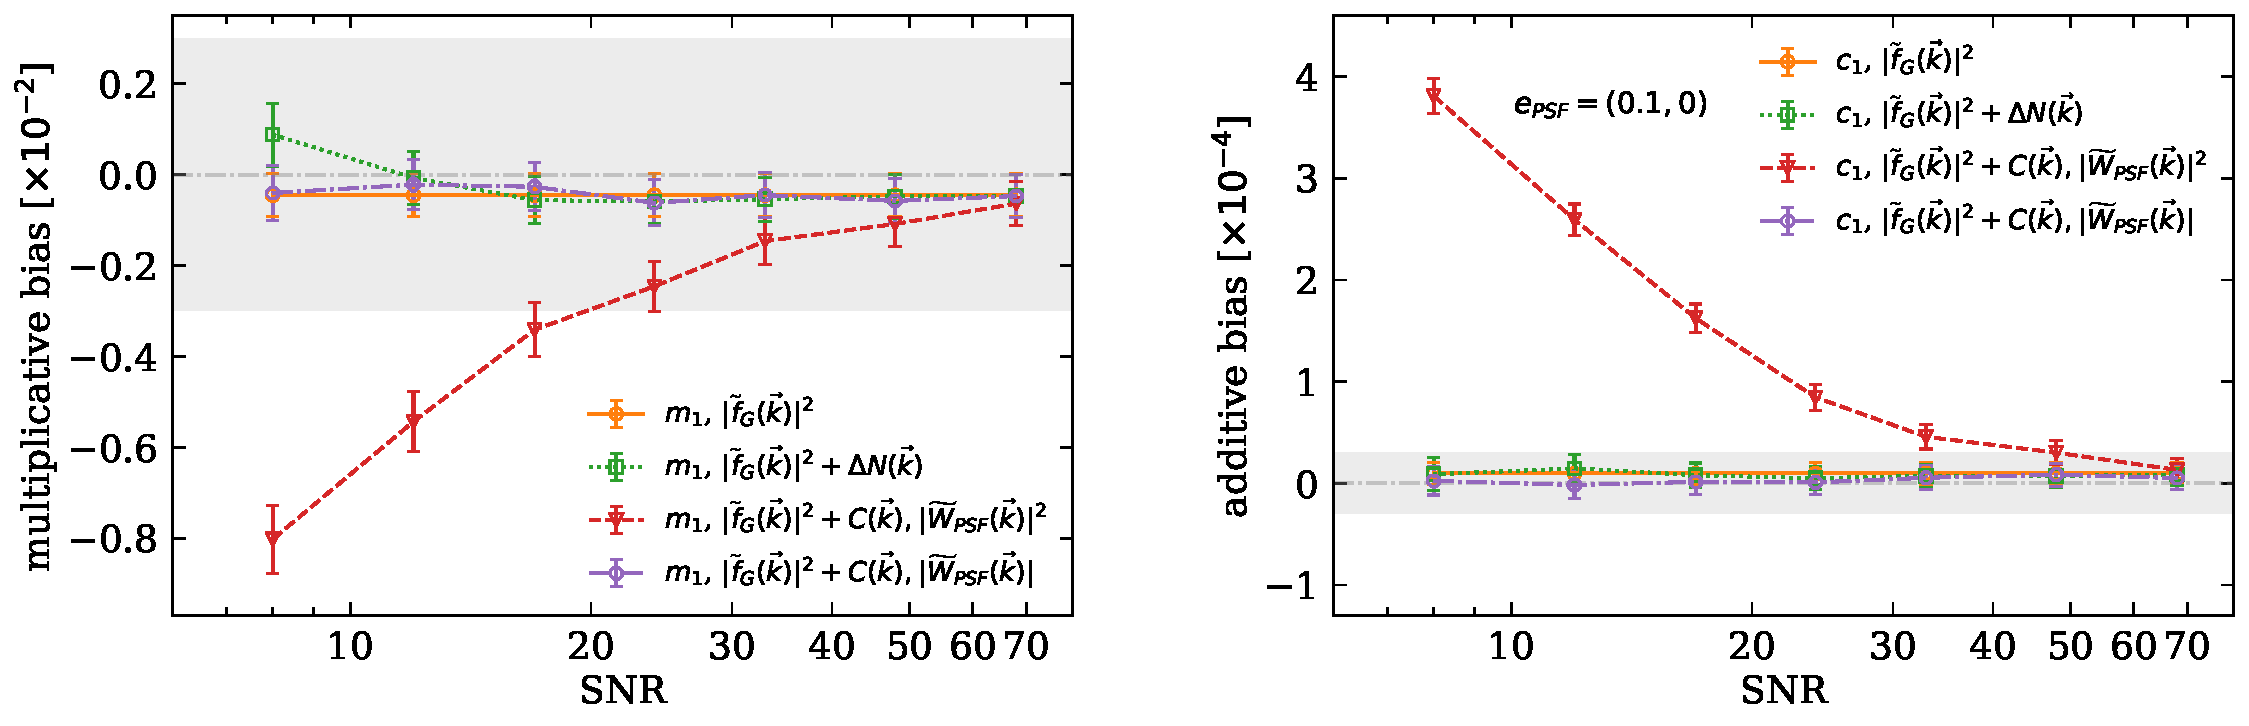
\includegraphics[width=0.9\linewidth]{figures/pts_sample_components.pdf}
	\caption{The multiplicative and additive bias measured from different components of the power spectrum of noisy galaxy image. Because the curves of $m_1$ and $m_2$ are very similar, only $m_1$ curves are presented. Only $c_1$'s are shown because all $c_2$'s are consistent with zero($e_{2}$ of PSF is zero)).  Orange curves: Measured from the power spectrum of noise free galaxy image. Green curves: Measured from the combination of noise free part and the noise power spectrum residual, $\Delta N(\vec{k})$. Red curves: Measured from the combination of noise free galaxy image power spectrum and the Fourier transform mixture, $C(\vec{k})$. The PSF power spectrum, $\vert \widetilde{W}_{PSF}(\vec{k})\vert^2$, is used for deconvolution. Purple curves: Same components are used for measurement as the red curves. However, $\vert \widetilde{W}_{PSF}(\vec{k})\vert$ is used (in $T(\vec{k})$) in PSF deconvolution for $C(\vec{k})$.}\label{fig:pts_componets}
\end{figure*}

\subsection{Improvement to the sub-percent precision}\label{sec:improve}
Although an appropriate PSF deconvolution for the $C(\vec{k})$ term would correct the bias, image components separation could not be achieved in the real data. It should be noted that what we have for measurement are the noisy images and the shear estimators measured from that. Among the components of $M(\vec{k})$, the $C(\vec{k})$ part is the one that easy to estimate. We propose a new method that utilizes the shear estimators from the estimated $C(\vec{k})$ to correct the bias. 

Recall that the original measurement, Eq.(\ref{FQ_TM}), employs the power spectrum of a noise image to subtract the contamination to shear estimators from the background noise. However, this operation leaves an annoying term, $C(\vec{k})$, to the shear measurement. In our new method, we need a second noise image, $f_{B^{\prime}}(\vec{x})$, to estimate this component. Then, we would get the shear estimators from this component by applying the shear measurement to it. There are three steps:
\begin{itemize}
	\item Add the second noise image to the original noisy galaxy image, $f_S(\vec{x})$, to get a new image, $f_{S^{\prime}}(\vec{x})$.
	\begin{eqnarray}
	f_{S^{\prime}}(\vec{x}) = f_G(\vec{x}) + f_N(\vec{x}) + f_{B^{\prime}}(\vec{x}).
	\end{eqnarray}
	
	\item Subtract the power spectrum of the new noise image and that of the original noisy galaxy image from the power spectrum of the new image above.
	\begin{eqnarray}
	C^{\prime}(\vec{k})=&&\left\vert \widetilde{f}_{S^{\prime}}(\vec{x})\right\vert^2 - \left\vert \widetilde{f}_{S}(\vec{x})\right\vert^2 - \left\vert \widetilde{f}_{B}(\vec{x})\right\vert^2 \\ \nonumber
	 =&& \widetilde{f}_{G}^{*}(\vec{k})\widetilde{f}_B(\vec{k}) + \widetilde{f}_{G}(\vec{k})\widetilde{f}_{B}^{*}(\vec{k}).
	\end{eqnarray}
	The noise-noise power mixture, $\widetilde{f}_{N}^{*}(\vec{k})\widetilde{f}_B(\vec{k}) + \widetilde{f}_{N}(\vec{k})\widetilde{f}_{B}^{*}(\vec{k})$, has been neglected because we find it would not change the result in our new method.
	
	\item Apply the shear measurement to $C^{\prime}$ to get the new shear estimator: $G_1^C$, $G_2^C$, $N^C$, $U^C$, and $V^C$.

\end{itemize}
The calculation of Section \ref{sec:bias_cal} indicates that the noise part in $C(\vec{k})$ is not import because it vanishes at last. Therefore, utilizing $C^{\prime}(\vec{k})$ is a promising way to solve this problem. 


use the formulae to show the way of correction by new crossing term

introduce the method to obtain the estimated crossing term \& apply to the simulated data

figure of the results of correction, random walk galaxies, SNR\_1 $\sim$ SNR\_n

figure of the same results from the Galsim galaxies, SNR\_1 $\sim$ SNR\_n

figure of a more realistic simulation, galaxies form faint to bright, separate the bright and faint sample

\section{conclusion}
\appendix
\section{Appendix A}\label{app_a}
\begin{equation}
P_N(N_k^{Re},N_k^{Im})=\frac{1}{2\pi\sigma^2}\exp\left[-\frac{\left(N_k^{Re}\right)^2+\left(N_k^{Im}\right)^2}{2\sigma^2}\right]
\end{equation}

\begin{eqnarray}
&P_G&\left(G_1,G_2\right)
=\frac{1}{(2\pi)^2}\frac{\pi}{\sqrt{C}}\exp\left[-\frac{D}{4C}\right].
\end{eqnarray}
The parameters are defined as:
\begin{eqnarray}
&C&=U_1U_3-U_2^2, \\ \nonumber
&D&=\left(G_1-\Gamma_1\right)^2U_3-2\left(G_1-\Gamma_1\right)\left(G_2-\Gamma_2\right)U_2 \\ \nonumber
&&+\left(G_2-\Gamma_2\right)^2U_1, \\ \nonumber
&&\left(\Gamma_1,\Gamma_2\right)=\Delta^2\sum_k\vert F_k\vert^2\left(A_k,B_k\right)\\ \nonumber
&&\left(U_1,U_2,U_3\right)=2\sigma^2\Delta^4\sum_k\vert F_k\vert^2\left(A_k^2,A_kB_k,B_k^2\right)\\ \nonumber
\end{eqnarray}
%It should be noted that $\vert F_k\vert^2$ in the $\Gamma$'s are slightly different from that in $U$'s. The former one comes from the power spectrum of noise free galaxy image. But the latter one comes from the $C(\vec{k})$ term.
\begin{eqnarray}
\Gamma_1&=&\int{d}^2\vec{k}\;P_k^{\prime}\exp(-\beta^2k^2)\vert F_S(\vec{k})\vert^2 \\ \nonumber
U_1&=&2\sigma^2\Delta^2\int{d}^2\vec{k} \; Q_k^{\prime}\exp(-2\beta^2k^2)\frac{\vert F_S(\vec{k})\vert^2}{\vert W_{PSF}(\mathrm{M}\vec{k})\vert^2}, \\ \nonumber
P_k^{\prime}&=&\left(1+4\beta^2g_2k_xk_y\right)\left(k_x^2-k_y^2\right), \\ \nonumber
Q_k^{\prime}&=&\left(1+8\beta^2g_2k_xk_y\right)\left(k_x^2-k_y^2\right)^2.
\end{eqnarray}


\section{Appendix B}\label{app_b}
\begin{thebibliography}{}

\bibitem[Rowe et al.(2015)]{Rowe2015}Rowe B, Jarvis M, Mandelbaum R, et al. \ 2015, A\&C, 10, 121

\bibitem[Zhang(2008)]{Zhang2008} Zhang J. \ 2008, \mnras, 383, 113


\bibitem[Zhang et al.(2015)]{Zhang2015} Zhang J, Luo W \& Sebastien F. \ 2015 \jcap, 1, 24

\bibitem[Zhang et al.(2017)]{Zhang2017} Zhang J, Zhang P, Luo W. \ 2017, \apj, 834, 8

\end{thebibliography}

\end{document}

% End of file `sample62.tex'.
